\newpage
\FloatBarrier
\section{Ogólne charakterystyki grafów}
\FloatBarrier
\subsection{Podstawowe miary}
\begin{figure}[h]
	\centering
	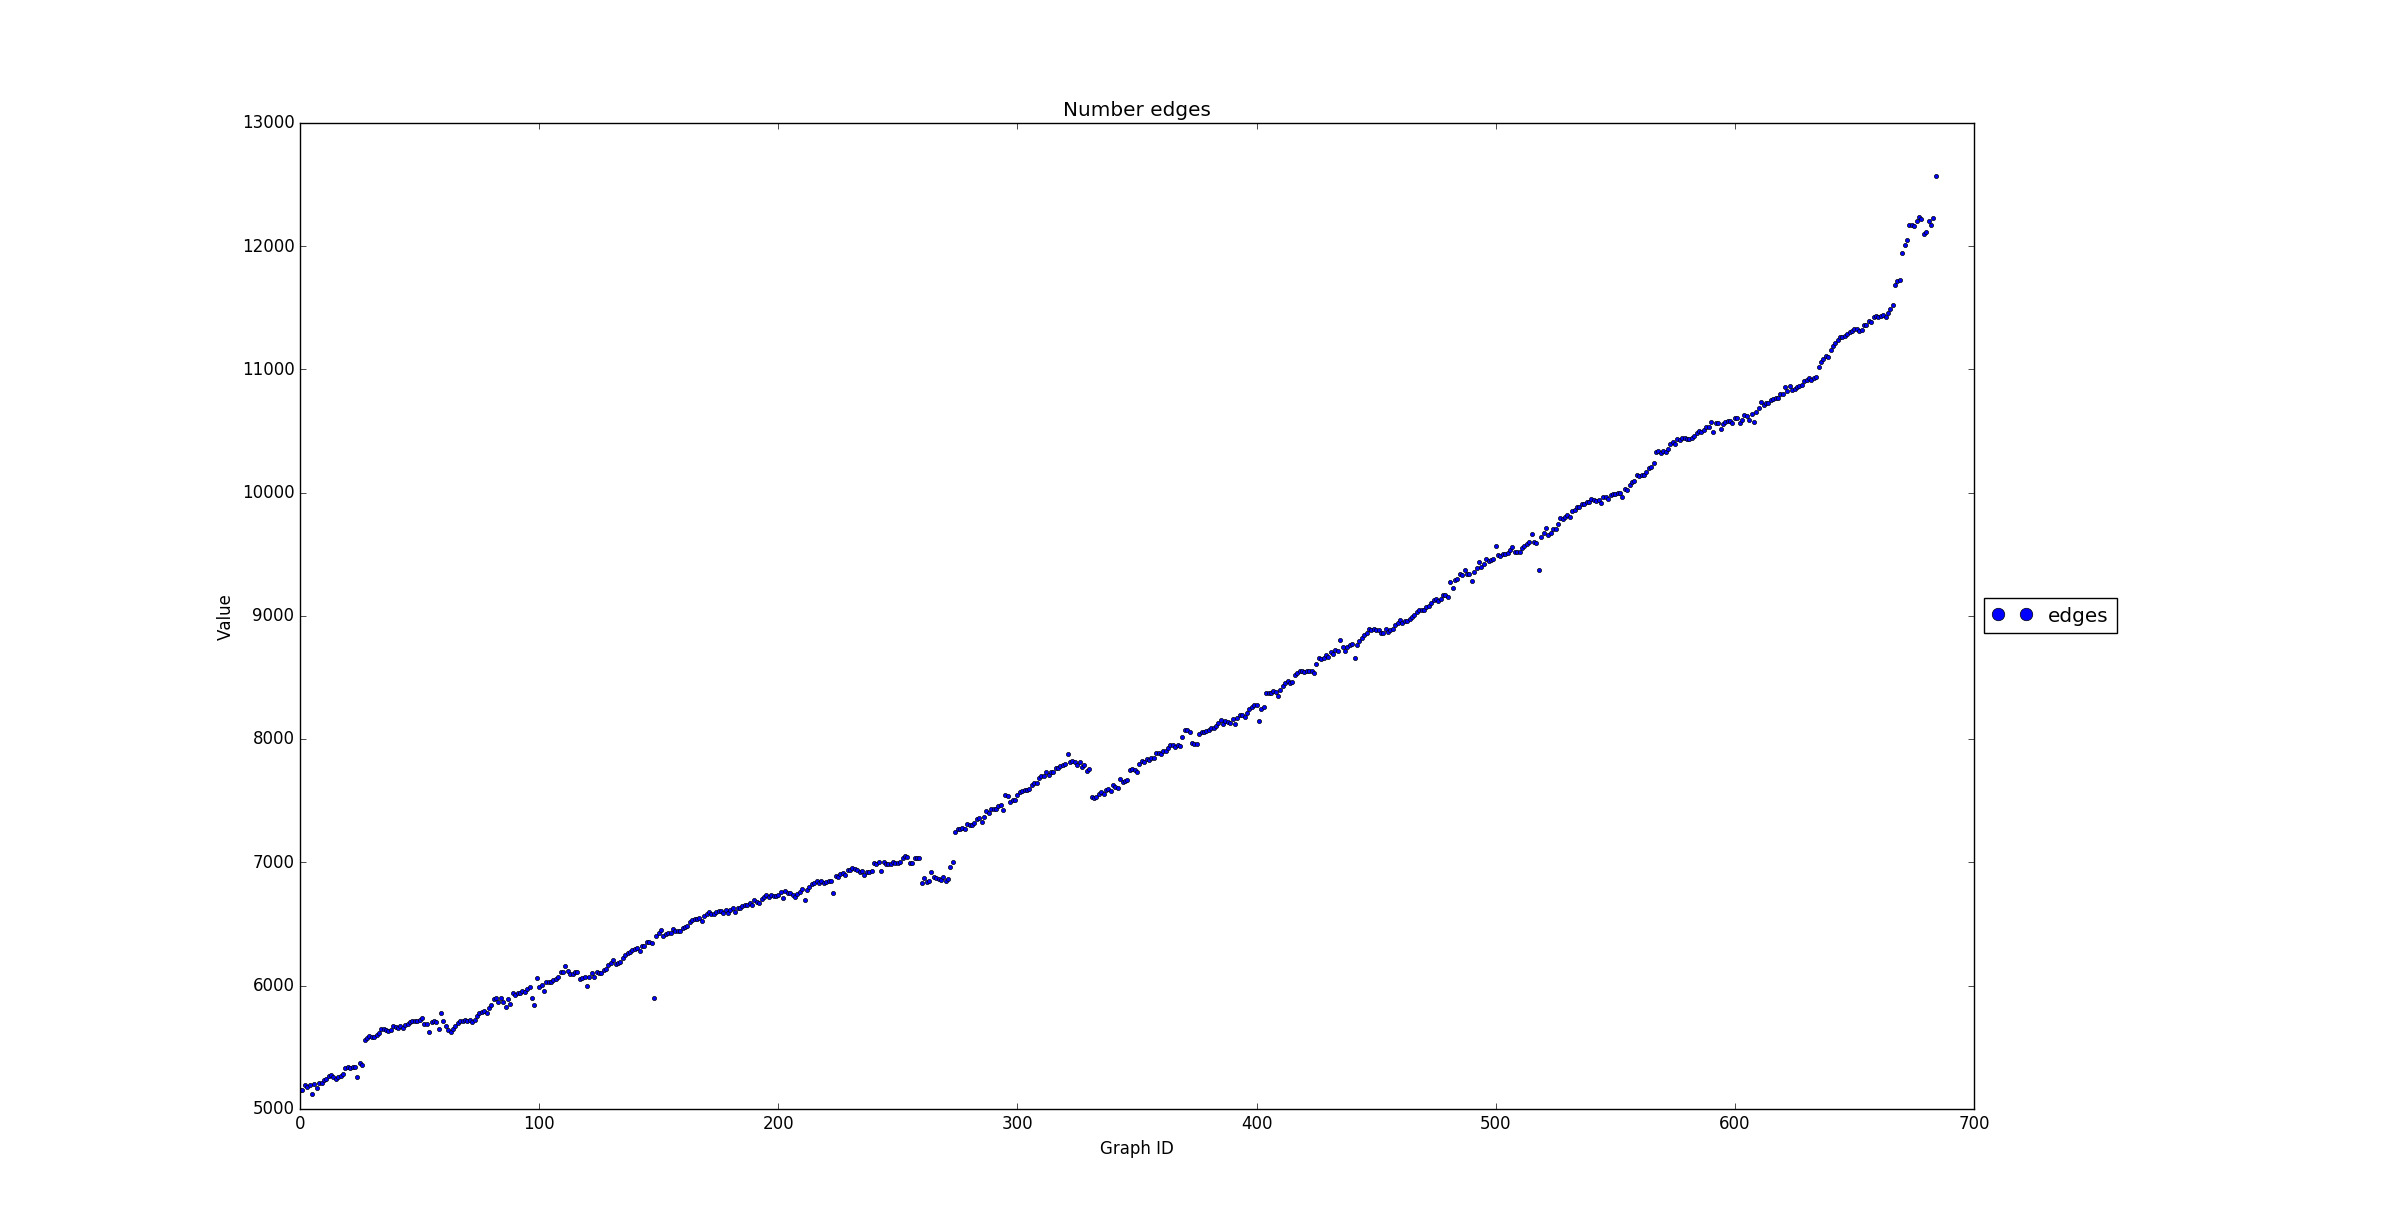
\includegraphics[width=\textwidth]{number_edges}
	\caption{Ilość krawędzi w sieci}
\end{figure}
\FloatBarrier
\FloatBarrier
\begin{figure}[h]
	\centering
	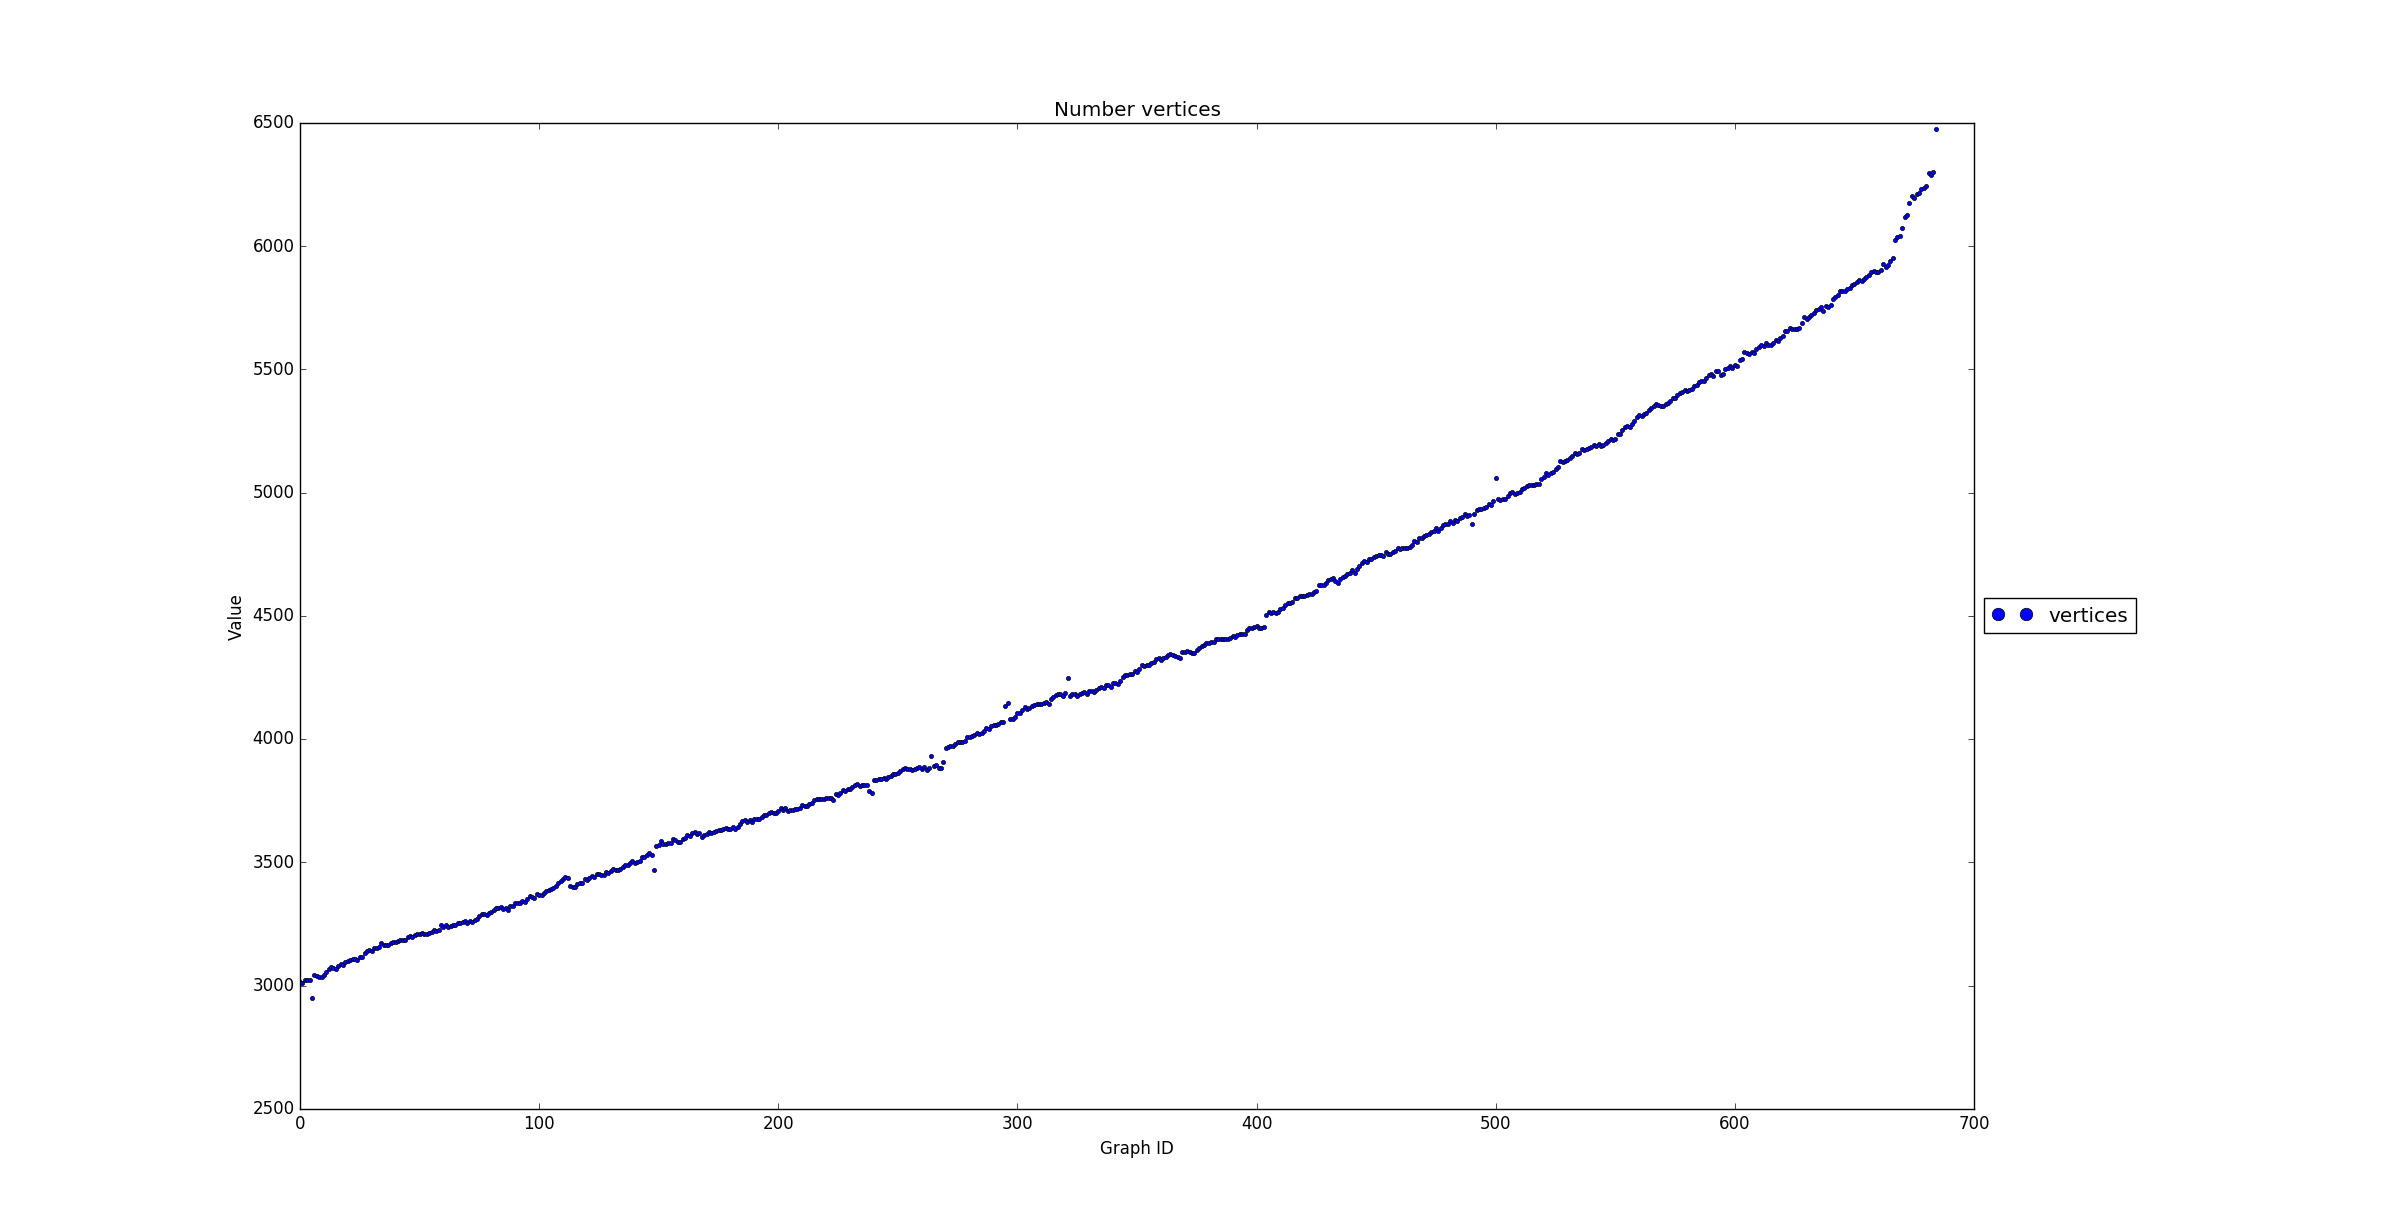
\includegraphics[width=\textwidth]{number_vertices}
	\caption{Ilość wierzchołków w sieci}
\end{figure}
\FloatBarrier
\FloatBarrier
\begin{figure}[h]
	\centering
	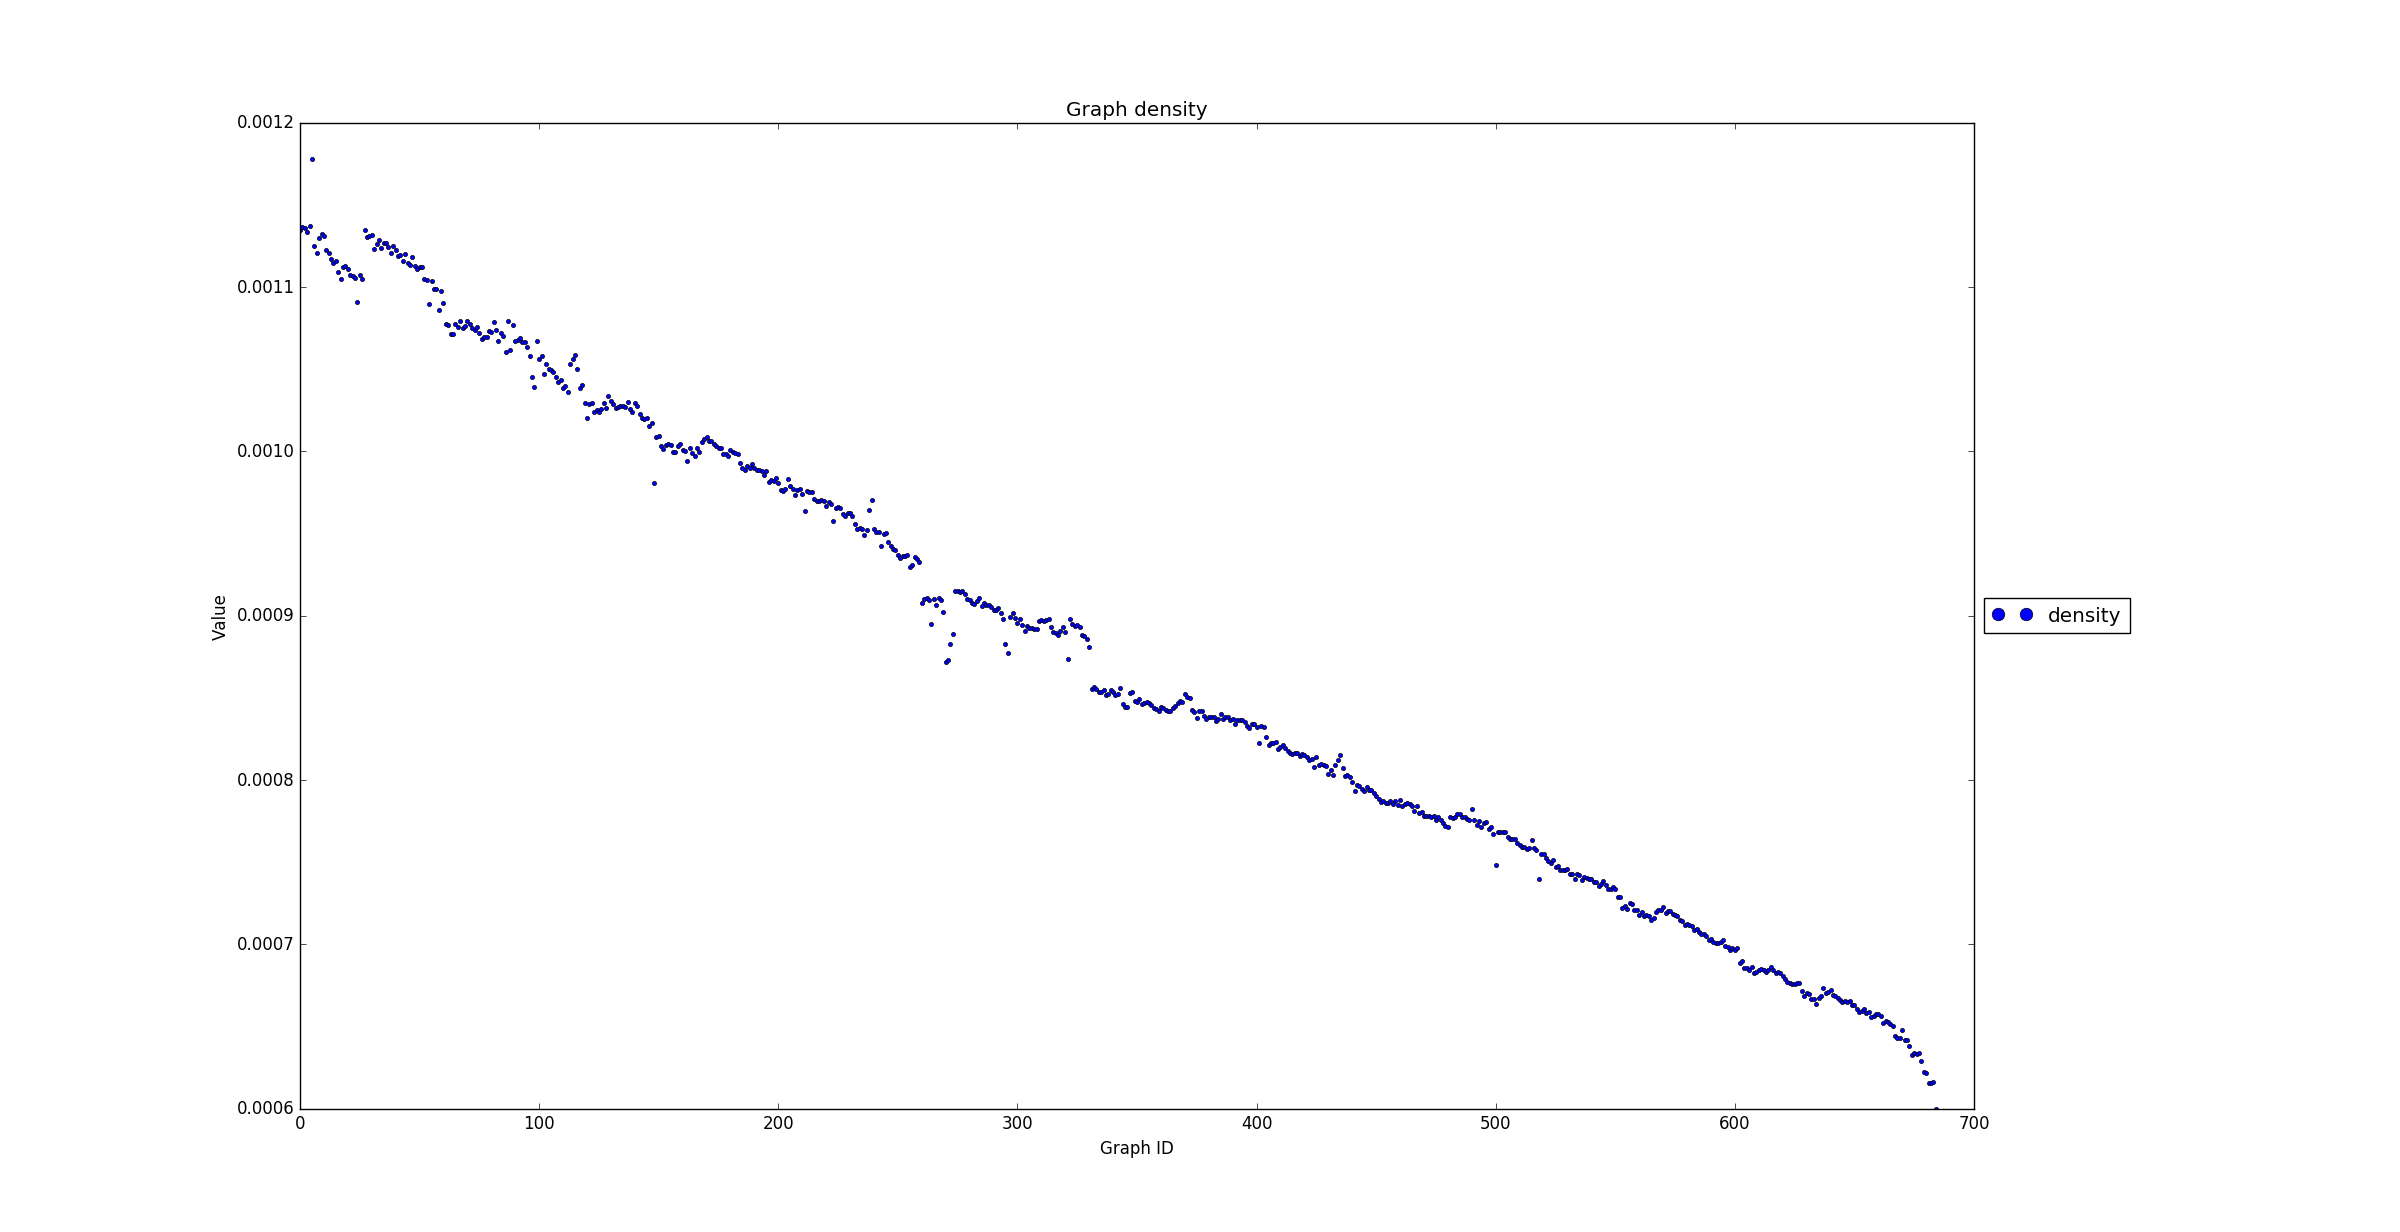
\includegraphics[width=\textwidth]{graph_density}
	\caption{Gęstość grafu}
\end{figure}
\FloatBarrier
Malejąca gęstość grafu wynika wprost z tego, że stosunek ilości wierzchołków do krawędzi jest stały w miarę upływu czasu, mimo tego że obie wartości rosną. Gęstość grafu liczymy ze wzoru:
\begin{equation}
\label{graph_density}
d=\frac{2m}{n(n-1)}
\end{equation}
$d$ - gęstość grafu, 
$m$ - ilość krawędzi, 
$n$ - ilość wierzchołków

Da się łatwo zauważyć, że jeśli stosunek $\frac{m}{n} = const$, a w tym przypadku $\frac{m}{n} \approx 2 \Rightarrow m \approx 2n$ to wzór \ref{graph_density} można zapisać następująco:
\begin{equation}
\label{graph_density_simplified}
d \approx \frac{4n}{n(n-1)} \equiv d \approx \frac{4}{n-1}
\end{equation}

Jak widać po przekształceniu uzyskujemy hiperbolę, którą dla dużych $n$ na wąskim przedziale $[3000, 6500]$ można przybliżyć malejącą funkcją liniową.
\FloatBarrier
\newpage